\documentclass{beamer}
\usepackage{animate}
\usepackage{amsmath}
\usepackage{tikz}
\usetheme{Madrid}

\setbeamercolor{structure}{fg=green!39!black} % changes main accent color to green

\useinnertheme{circles}
%Information to be included in the title page:
\title{Measuring Changes in Pol II Speed \& Splicing Time}
\author{Jakub Koubele}
\institute{Progress Report}
\date{9th September, 2025}

\renewcommand{\insertshortauthor}{Jakub Koubele}  
\renewcommand{\insertshorttitle}{Pol II speed and splicing}
\renewcommand{\insertshortdate}{9th September, 2025} % Define custom text for 3rd block

\usepackage{amsthm}
\newcommand*{\QED}{\hfill\ensuremath{\blacksquare}}





\begin{document}
	\frame{\titlepage}
	
	
	\begin{frame}
		\frametitle{Introduction}	
		\pause
		
		\begin{itemize}
			\item A pre-print of this work is available on BioRxiv.
			
			\begin{center}
			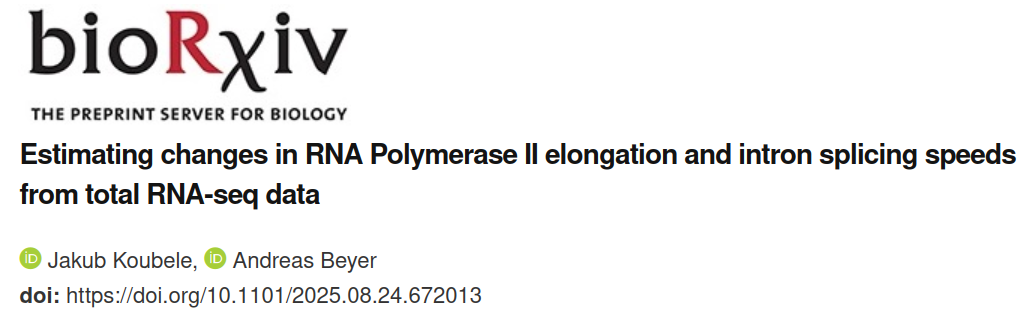
\includegraphics[scale=0.32]{biorxiv_2}	
			\end{center}	
			
			\pause
			
			\item Presentation outline:
			\begin{itemize}
				\item Model derivation
				\item Fitting and statistical inference
				\item Implementation details
				
			\end{itemize}
			
		\end{itemize}		
		
	\end{frame}
	
	
	\begin{frame}
		\frametitle{Model overview}	
		\pause
		
		\begin{itemize}
			\item The model works with total (ribo-minus) RNA-seq data.
			\pause
			
			\item The model consists of inputs, outputs, and parameters. 
			\pause
			
			\item \textbf{Inputs} are the vectors of explanatory variables (sample annotation), denoted $\mathbf{x}$.
			\pause
			
			\item \textbf{Parameters} are the LFC of gene expression, Pol II speed, and intron splicing time.
			\begin{itemize}
				\item Several intercept terms are also included.
			\end{itemize}
			\pause
			
			\item \textbf{Outputs} are the predicted exon and intron read counts, and location of reads within introns (coverage).			
			
		\end{itemize}		
	\end{frame}
	
	\begin{frame}
		\frametitle{Total RNA-seq illustration}	
		\pause
		\begin{center}
			
\includegraphics[scale=0.25]{total_rna}	
		\end{center}
	\end{frame}
	
	\begin{frame}
		\frametitle{Data pre-processing}	
		\pause
		\begin{itemize}
			\item The reads are aligned to the genome. We construct count matrix for introns (by counting overlapping reads).
			\pause
			\begin{itemize}
				\item For each intron, we also record its coverage (i.e. read histogram).
			\end{itemize}
			\pause
			\item Reads not overlapping with any intron are aligned to the transcriptome, and used to construct a gene-level exon count matrix.
			
		\end{itemize}
		
	\end{frame}
	
	
	\begin{frame}
		\frametitle{Modeled gene properties}	
		\pause
		\begin{itemize}
			\item \textbf{Expression rate} (gene-specific):    
			$$
			\eta = \eta_0 \exp \left( \mathbf{x}^\mathsf{T} \boldsymbol{\alpha} \right)
			$$
			The unit is $\left[ \eta\right] = \mathrm{polymerases} \cdot \mathrm{s}^{-1}$. The parameter $\boldsymbol{\alpha}$ is a vector with the LFC of expression rate.
			\pause
			
			\item \textbf{Pol II speed} (intron-specific):
			$$
			v = v_0 \exp \left( \mathbf{x}^\mathsf{T} \boldsymbol{\beta} \right)
			$$ 
			The unit is $\left[ v \right] = \mathrm{bp} \cdot \mathrm{s}^{-1}$. The parameter $\boldsymbol{\beta}$ is a vector with the LFC of Pol II speed.
			\pause
			
			\item \textbf{Splicing time} (intron-specific):
			$$
			\tau = \tau_0 \exp \left( \mathbf{x}^\mathsf{T} \boldsymbol{\gamma} \right)
			$$ 
			The unit is $\left[ \tau \right] = \mathrm{s}$. The parameter $\boldsymbol{\gamma}$ is a vector with the LFC of splicing time.
			
		\end{itemize}
	\end{frame}
	
	
	\begin{frame}
		\frametitle{Predicting exon read count}	
		\pause
		\begin{itemize}
			\item We predict the exon read count as
			$$
			\mu =  \exp \left( \text{intercept}_{\text{exons}} + \mathbf{x}^\mathsf{T} \boldsymbol{\alpha} \right)
			$$ 
			i.e. the exon reads simply scale with the gene expression rate.
			\pause
			\item Two caveats:
			\begin{itemize}
				\item Small fraction of exonic reads are from nascent RNA; their amount thus also depend on Pol II speed. 
				\pause
				
				\item Transcript abundance is also affected by the degradation rate (transcript half-life).
			\end{itemize}
		\end{itemize}
		\end{frame}
		
	\begin{frame}
		\frametitle{Transcribing and unspliced introns}	
		\pause
		\begin{itemize}
			\item The intronic reads come from two sources: currently transcribing introns, and finished introns which are not spliced yet.
			\pause
			\item Number of reads from transcribing introns scales with the gene expression rate, and with the time needed to transcribe the intron:
			$$
			n_{\text{transcribing}} \propto \eta L v^{-1}
			$$
			where L the intron length, $\left[ L \right] = \mathrm{bp}$.
			\pause
			\item Number of reads from unspliced introns scales with the gene expression rate, and with the time needed to splice out the intron:
			$$
			n_{\text{unspliced}} \propto \eta \tau
			$$
			
		\end{itemize}
	\end{frame}
	
	
	\begin{frame}
		\frametitle{Predicting intron read count}	
		\pause
		\begin{itemize}
			\item The number of intronic reads depends on transcribing and unspliced introns as
			$$\nu \propto n_{\text{transcribing}} +2 \cdot n_{\text{unspliced}}$$
			\pause 
			\item After plugging in the values from gene properties definitions, we get:
			\pause
			
		
			
			\begin{align*}
				\nu \propto & \exp \left( \log \left(2 \tau_{0} \eta_0 \right) + \theta 
				+ \mathbf{x}^\mathsf{T} \left( \boldsymbol{\alpha} - \boldsymbol{\beta} \right) \right) \\
				&+ \exp \left( \log \left(2 \tau_{0} \eta_0 \right) 
				+  \mathbf{x}^\mathsf{T} \left( \boldsymbol{\alpha} + \boldsymbol{\gamma} \right) \right)
			\end{align*}
			where
			$$
			\theta = \log \left( \frac{1}{2} Lv_0^{-1} \tau_0^{-1} \right)
			$$
			\pause
			\item By introducing an intercept term, we obtain:			
			{\small
				\[
				\nu = \exp \left(\text{intercept}_{\text{intron}} + \theta 
				+ \mathbf{x}^\mathsf{T} \left( \boldsymbol{\alpha} - \boldsymbol{\beta} \right) \right)
				+ \exp \left( \text{intercept}_{\text{intron}} 
				+ \mathbf{x}^\mathsf{T} \left( \boldsymbol{\alpha} + \boldsymbol{\gamma} \right) \right)
				\]
			}			
			
		\end{itemize}
	\end{frame}
	
	\begin{frame}
		\frametitle{Effect of Pol II speed change illustration}	
		\pause
		\begin{center}	
			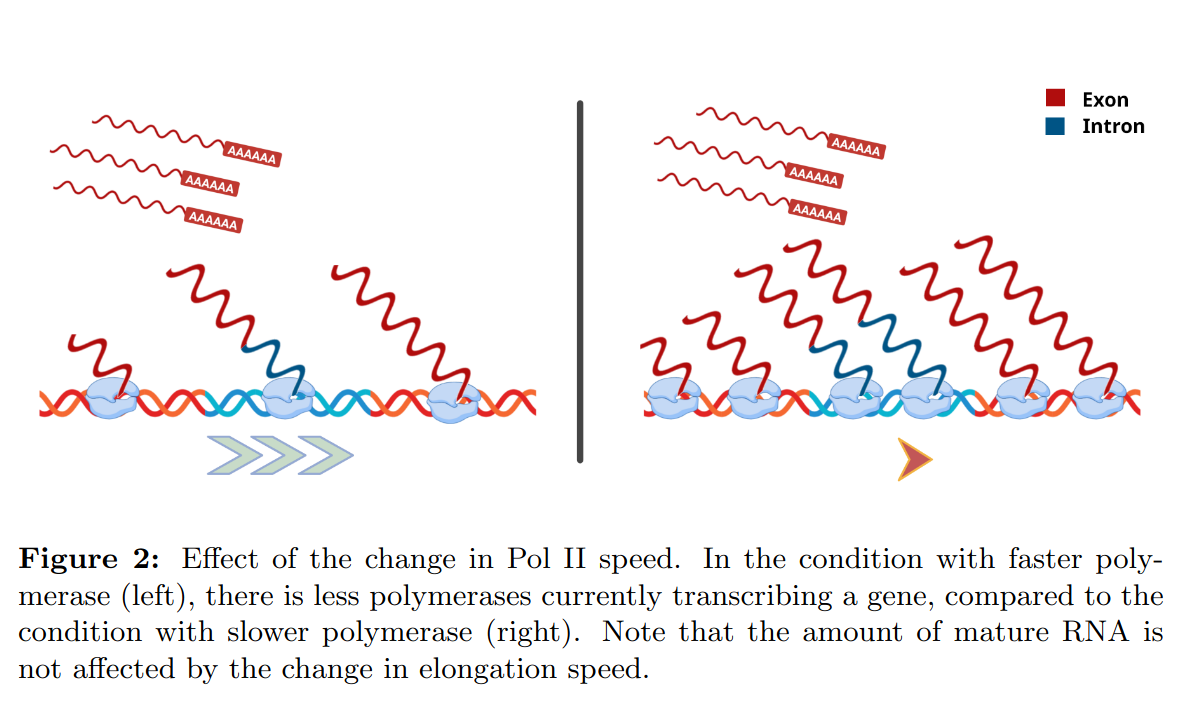
\includegraphics[scale=0.27]{speed_effect.png}
		\end{center}
	\end{frame}
	
	
	\begin{frame}
		\frametitle{Intron coverage density}	
		\small
		\pause
		\begin{itemize}
			\item For simplicity, assume the intron to be a continuous interval $[0, 1]$, oriented in the 5’ to 3’ direction.
			\pause
			\item Unspliced introns can produce reads anywhere in the intron. Their location then  follows a uniform distribution, with the density
			$$
			p_U(r) = 1, \quad r \in [0,1]   
			$$\pause
			\item Transcribing introns can produce reads only in the part
			of the intron that was already transcribed. We model their location by a decreasing triangular density
			$$
			p_T(r) = 2-2r, \quad r \in [0,1]   
			$$\pause			
			\item The overall distribution of intronic reads is then a mixture of the uniform and triangular components, with the density
			$$
			p(r) = \pi p_T(r) + (1-\pi) p_U(r) = 1 +\pi -2\pi r, \quad r \in [0,1]   
			$$ 
			Where $\pi \in [0,1]$ is the mixture weight of the triangular distribution.
			
		\end{itemize}
	\end{frame}
	
		\begin{frame}
		\frametitle{Intron coverage density illustartion}	
		\pause
		\begin{center}	
			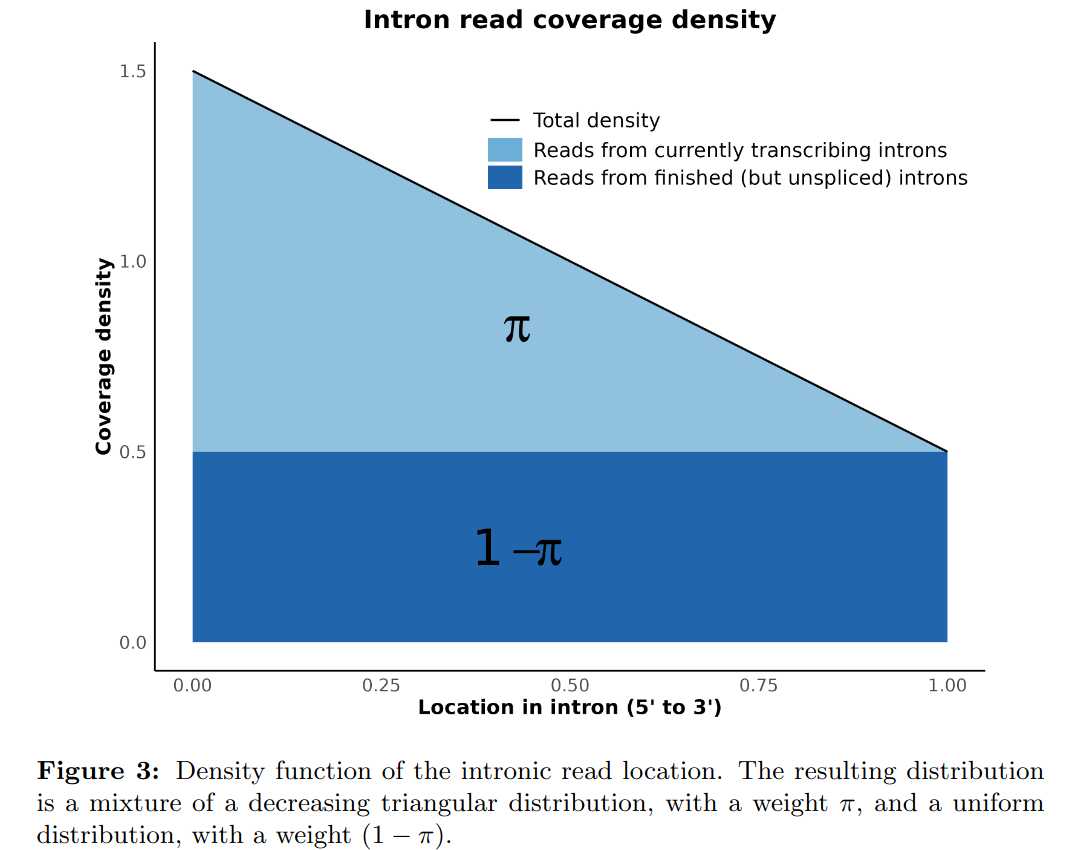
\includegraphics[scale=0.25]{density.png}
		\end{center}
	\end{frame}
	
		
	\begin{frame}
		\frametitle{Predicting intron reads location}
		\pause
		\begin{itemize}
			\item The mixture parameter $\pi$ depends on the number of reads from transcribing and unspliced introns:
			$$
			\pi = \frac{n_{\text{transcribing}}}{n_{\text{transcribing}} + 2 \cdot n_{\text{unspliced}}}
			$$
			\pause
			\item After plugging in the formulas from definitions, we arrive to 
			$$
			\pi = \frac{\exp \left( \theta -\mathbf{x}^\mathsf{T} \left( \boldsymbol{\beta} + \boldsymbol{\gamma} \right)  \right)}{1 + \exp \left( \theta -\mathbf{x}^\mathsf{T} \left( \boldsymbol{\beta} + \boldsymbol{\gamma} \right)  \right)}
			= \sigma \left( \theta -\mathbf{x}^\mathsf{T} \left( \boldsymbol{\beta} + \boldsymbol{\gamma} \right) \right)
			$$ 
			where $\sigma(.)$ denotes the logistic (sigmoid) function.
		\end{itemize}
	\end{frame}
	
	
	
	\begin{frame}
		\frametitle{The End}
		Thank you for your attention!
		\begin{center}	
			
\includegraphics[scale=0.07]{group_picture.png}
		\end{center}
		
		\tiny{Illustrations were created using BioRender.}
	\end{frame}

	
	
\end{document}
